% Backup — Dispersão de CTI por política (figura isolada, slide original do Capítulo 6)
\begin{frame}[noframenumbering]{[Backup] Dispersão de CTI por política}
  \centering
  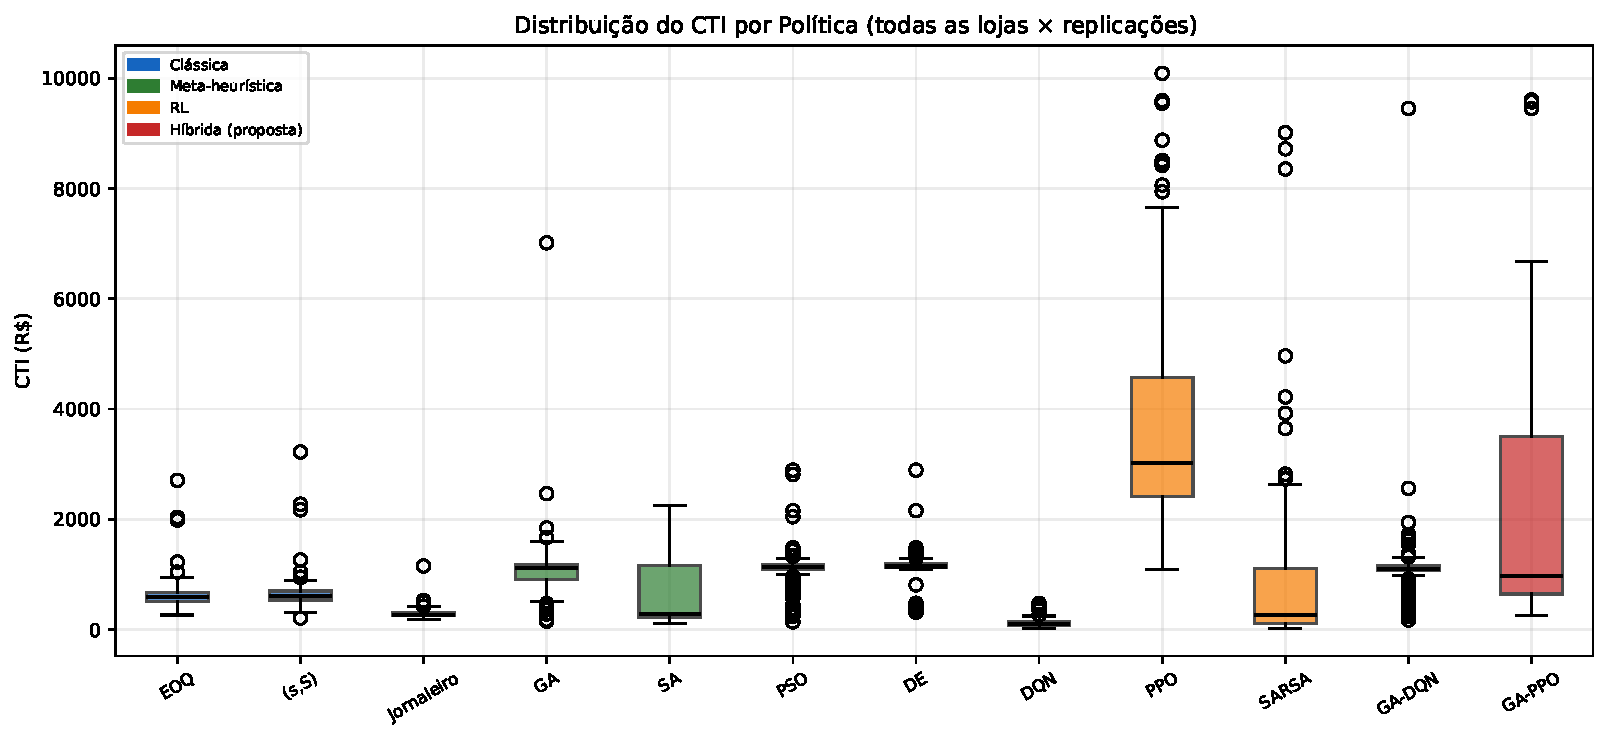
\includegraphics[width=0.62\linewidth,height=6.6cm,keepaspectratio]{figures/boxplot_tic.pdf}\\[0.4em]
  {\small Distribuição do CTI por política (boxplot sobre as 145 séries).}
  \note{
    Este boxplot mostra a distribuição de CTI de cada política sobre as 145
    séries. Caixas mais altas indicam que a mesma política produz custos
    muito diferentes entre séries -- a eficácia depende do perfil da
    demanda, não apenas da política escolhida. Algumas políticas, como GA,
    GA-DQN e GA-PPO, têm coeficiente de variação de CTI acima de 100\% entre
    séries. (Slide de backup: detalha a dispersão por política, caso a
    banca peça mais evidência além da fronteira de Pareto do corpo
    principal.)
  }
\end{frame}
